% SPDX-FileCopyrightText: Contributors to PyPSA-Wal
% SPDX-License-Identifier: CC-BY-4.0
%
% Compiled by workflow_pv_wal/Snakefile (rule build_report, tectonic).
% Every number in this document comes from generated/macros.tex; do not type
% figures by hand.

\documentclass[11pt,a4paper]{article}

\usepackage[T1]{fontenc}
\usepackage[utf8]{inputenc}
\usepackage[english]{babel}
\usepackage{lmodern}
\usepackage{textcomp}
\usepackage[section]{placeins}
\usepackage{microtype}
\usepackage[margin=2.4cm]{geometry}
\usepackage{graphicx}
\usepackage{booktabs}
\usepackage{longtable}
\usepackage{siunitx}
\usepackage{xcolor}
\usepackage{enumitem}
\usepackage{caption}
\usepackage{fancyhdr}
\usepackage[htt]{hyphenat}
\usepackage[hidelinks]{hyperref}

\emergencystretch=3em
\hyphenpenalty=1000

\sisetup{group-separator={\,},group-minimum-digits=4,detect-all}
\captionsetup{font=small,labelfont=bf}
\setlist{nosep,leftmargin=*}

\definecolor{wal}{HTML}{2B8A3E}
\definecolor{warn}{HTML}{C92A2A}
\newcommand{\finding}[1]{\par\medskip\noindent\colorbox{wal!10}{%
  \begin{minipage}{\dimexpr\linewidth-2\fboxsep}\textbf{Finding.} #1\end{minipage}}\par\medskip}
\newcommand{\caveat}[1]{\par\medskip\noindent\colorbox{warn!8}{%
  \begin{minipage}{\dimexpr\linewidth-2\fboxsep}\textbf{Caveat.} #1\end{minipage}}\par\medskip}

\pagestyle{fancy}
\fancyhf{}
\fancyhead[L]{\small Walloon ground-mounted PV technical potential}
\fancyhead[R]{\small PyPSA-Wal}
\fancyfoot[C]{\thepage}
\renewcommand{\headrulewidth}{0.3pt}

% Generated by workflow_pv_wal/scripts/make_report_inputs.py -- do not edit.
\newcommand{\RegionKm}{16\,905}
\newcommand{\GridRes}{20}
\newcommand{\LeftNatureKm}{14\,490}
\newcommand{\LeftNaturePct}{85.7}
\newcommand{\DropNatureKm}{2\,416}
\newcommand{\LeftForestKm}{10\,788}
\newcommand{\LeftForestPct}{63.8}
\newcommand{\DropForestKm}{3\,701}
\newcommand{\LeftCoverKm}{10\,040}
\newcommand{\LeftCoverPct}{59.4}
\newcommand{\DropCoverKm}{748}
\newcommand{\LeftLandscapeKm}{9\,185}
\newcommand{\LeftLandscapePct}{54.3}
\newcommand{\DropLandscapeKm}{855}
\newcommand{\LeftHazardKm}{9\,027}
\newcommand{\LeftHazardPct}{53.4}
\newcommand{\DropHazardKm}{157}
\newcommand{\LeftTerrainKm}{7\,927}
\newcommand{\LeftTerrainPct}{46.9}
\newcommand{\DropTerrainKm}{1\,100}
\newcommand{\LeftBuiltKm}{6\,993}
\newcommand{\LeftBuiltPct}{41.4}
\newcommand{\DropBuiltKm}{934}
\newcommand{\LeftWaterKm}{6\,971}
\newcommand{\LeftWaterPct}{41.2}
\newcommand{\DropWaterKm}{23}
\newcommand{\LeftParkRuleKm}{6\,275}
\newcommand{\LeftParkRulePct}{37.1}
\newcommand{\DropParkRuleKm}{696}
\newcommand{\FloatHa}{2\,057}
\newcommand{\GWaterIndustrialEligHa}{544}
\newcommand{\GWaterIndustrialTechHa}{544}
\newcommand{\GWaterIndustrialOpenHa}{544}
\newcommand{\GWaterIndustrialTechMW}{204}
\newcommand{\GWaterIndustrialTechGW}{0.2}
\newcommand{\GWaterIndustrialRefMW}{204}
\newcommand{\GWaterOtherEligHa}{1\,514}
\newcommand{\GWaterOtherTechHa}{1\,514}
\newcommand{\GWaterOtherOpenHa}{0}
\newcommand{\GWaterOtherTechMW}{568}
\newcommand{\GWaterOtherTechGW}{0.6}
\newcommand{\GWaterOtherRefMW}{0}
\newcommand{\GCetEligHa}{99}
\newcommand{\GCetTechHa}{66}
\newcommand{\GCetOpenHa}{65}
\newcommand{\GCetTechMW}{66}
\newcommand{\GCetTechGW}{0.1}
\newcommand{\GCetRefMW}{65}
\newcommand{\GSarEligHa}{1\,768}
\newcommand{\GSarTechHa}{967}
\newcommand{\GSarOpenHa}{861}
\newcommand{\GSarTechMW}{967}
\newcommand{\GSarTechGW}{1.0}
\newcommand{\GSarRefMW}{861}
\newcommand{\GTerrilEligHa}{121}
\newcommand{\GTerrilTechHa}{47}
\newcommand{\GTerrilOpenHa}{41}
\newcommand{\GTerrilTechMW}{47}
\newcommand{\GTerrilTechGW}{0.0}
\newcommand{\GTerrilRefMW}{41}
\newcommand{\GQuarryActiveEligHa}{1\,564}
\newcommand{\GQuarryActiveTechHa}{981}
\newcommand{\GQuarryActiveOpenHa}{0}
\newcommand{\GQuarryActiveTechMW}{981}
\newcommand{\GQuarryActiveTechGW}{1.0}
\newcommand{\GQuarryActiveRefMW}{0}
\newcommand{\GAgriGrasslandPermEligHa}{186\,751}
\newcommand{\GAgriGrasslandPermTechHa}{173\,872}
\newcommand{\GAgriGrasslandPermOpenHa}{3\,781}
\newcommand{\GAgriGrasslandPermTechMW}{121\,711}
\newcommand{\GAgriGrasslandPermTechGW}{121.7}
\newcommand{\GAgriGrasslandPermRefMW}{2\,647}
\newcommand{\GAgriGrasslandTempEligHa}{31\,121}
\newcommand{\GAgriGrasslandTempTechHa}{30\,178}
\newcommand{\GAgriGrasslandTempOpenHa}{652}
\newcommand{\GAgriGrasslandTempTechMW}{21\,125}
\newcommand{\GAgriGrasslandTempTechGW}{21.1}
\newcommand{\GAgriGrasslandTempRefMW}{456}
\newcommand{\GAgriArableEligHa}{323\,174}
\newcommand{\GAgriArableTechHa}{319\,046}
\newcommand{\GAgriArableOpenHa}{0}
\newcommand{\GAgriArableTechMW}{111\,666}
\newcommand{\GAgriArableTechGW}{111.7}
\newcommand{\GAgriArableRefMW}{0}
\newcommand{\GAgriPerennialEligHa}{3\,175}
\newcommand{\GAgriPerennialTechHa}{3\,099}
\newcommand{\GAgriPerennialOpenHa}{0}
\newcommand{\GAgriPerennialTechMW}{1\,860}
\newcommand{\GAgriPerennialTechGW}{1.9}
\newcommand{\GAgriPerennialRefMW}{0}
\newcommand{\GAgriOtherEligHa}{7\,378}
\newcommand{\GAgriOtherTechHa}{6\,938}
\newcommand{\GAgriOtherOpenHa}{0}
\newcommand{\GAgriOtherTechMW}{4\,856}
\newcommand{\GAgriOtherTechGW}{4.9}
\newcommand{\GAgriOtherRefMW}{0}
\newcommand{\GExtractionEligHa}{969}
\newcommand{\GExtractionTechHa}{693}
\newcommand{\GExtractionOpenHa}{495}
\newcommand{\GExtractionTechMW}{693}
\newcommand{\GExtractionTechGW}{0.7}
\newcommand{\GExtractionRefMW}{495}
\newcommand{\GInfraEdgeEligHa}{2\,728}
\newcommand{\GInfraEdgeTechHa}{949}
\newcommand{\GInfraEdgeOpenHa}{226}
\newcommand{\GInfraEdgeTechMW}{949}
\newcommand{\GInfraEdgeTechGW}{0.9}
\newcommand{\GInfraEdgeRefMW}{226}
\newcommand{\GZaeEligHa}{5\,141}
\newcommand{\GZaeTechHa}{2\,788}
\newcommand{\GZaeOpenHa}{584}
\newcommand{\GZaeTechMW}{2\,788}
\newcommand{\GZaeTechGW}{2.8}
\newcommand{\GZaeRefMW}{584}
\newcommand{\GZspecEligHa}{5\,160}
\newcommand{\GZspecTechHa}{2\,762}
\newcommand{\GZspecOpenHa}{535}
\newcommand{\GZspecTechMW}{2\,762}
\newcommand{\GZspecTechGW}{2.8}
\newcommand{\GZspecRefMW}{535}
\newcommand{\GAgriZonePoorEligHa}{5\,281}
\newcommand{\GAgriZonePoorTechHa}{4\,697}
\newcommand{\GAgriZonePoorOpenHa}{140}
\newcommand{\GAgriZonePoorTechMW}{4\,697}
\newcommand{\GAgriZonePoorTechGW}{4.7}
\newcommand{\GAgriZonePoorRefMW}{140}
\newcommand{\GAgriZoneUnfarmedEligHa}{57\,807}
\newcommand{\GAgriZoneUnfarmedTechHa}{50\,304}
\newcommand{\GAgriZoneUnfarmedOpenHa}{0}
\newcommand{\GAgriZoneUnfarmedTechMW}{50\,304}
\newcommand{\GAgriZoneUnfarmedTechGW}{50.3}
\newcommand{\GAgriZoneUnfarmedRefMW}{0}
\newcommand{\GHabitatEligHa}{63\,962}
\newcommand{\GHabitatTechHa}{29\,721}
\newcommand{\GHabitatOpenHa}{0}
\newcommand{\GHabitatTechMW}{29\,721}
\newcommand{\GHabitatTechGW}{29.7}
\newcommand{\GHabitatRefMW}{0}
\newcommand{\GOtherEligHa}{841}
\newcommand{\GOtherTechHa}{399}
\newcommand{\GOtherOpenHa}{0}
\newcommand{\GOtherTechMW}{399}
\newcommand{\GOtherTechGW}{0.4}
\newcommand{\GOtherRefMW}{0}
\newcommand{\RefMW}{6\,254}
\newcommand{\RefGW}{6.3}
\newcommand{\RefHa}{7\,924}
\newcommand{\TechMW}{356\,362}
\newcommand{\TechGW}{356}
\newcommand{\TechNonAgriGW}{95.1}
\newcommand{\TechAgriGW}{261}
\newcommand{\TechAgriHa}{533\,133}
\newcommand{\TechAgriShareSau}{72}
\newcommand{\RefCapHa}{4\,434}
\newcommand{\RefDegradedGW}{1.9}
\newcommand{\RefZaeGW}{1.1}
\newcommand{\RefZaeShare}{25}
\newcommand{\ParkMinHa}{1}
\newcommand{\ParkMinWidth}{60}
\newcommand{\DensGround}{1.00}
\newcommand{\DensGroundLow}{0.70}
\newcommand{\DensGroundHigh}{1.40}
\newcommand{\DensAgrivoltaicGrazing}{0.70}
\newcommand{\DensAgrivoltaicGrazingLow}{0.50}
\newcommand{\DensAgrivoltaicGrazingHigh}{0.80}
\newcommand{\DensAgrivoltaicCrops}{0.35}
\newcommand{\DensAgrivoltaicCropsLow}{0.25}
\newcommand{\DensAgrivoltaicCropsHigh}{0.50}
\newcommand{\DensAgrivoltaicCanopy}{0.60}
\newcommand{\DensAgrivoltaicCanopyLow}{0.40}
\newcommand{\DensAgrivoltaicCanopyHigh}{0.70}
\newcommand{\DensFloating}{1.50}
\newcommand{\DensFloatingLow}{1.00}
\newcommand{\DensFloatingHigh}{2.00}
\newcommand{\FloatCover}{25}
\newcommand{\SlopeMax}{15}
\newcommand{\NorthMax}{7}
\newcommand{\BuiltPct}{20}
\newcommand{\SealedPct}{50}
\newcommand{\TreesPct}{50}
\newcommand{\SauHa}{738\,927}
\newcommand{\SauKha}{739}
\newcommand{\EvShare}{5.1}
\newcommand{\EvMappedPoorHa}{4\,697}
\newcommand{\EvNotLpisHa}{2\,754}
\newcommand{\EvNotCurtilageHa}{2\,245}
\newcommand{\EvRevealedWeightedHa}{241}
\newcommand{\EvFarmedClassOne}{91}
\newcommand{\EvFarmedClassTwo}{89}
\newcommand{\EvFarmedClassThree}{88}
\newcommand{\EvFarmedClassFour}{93}
\newcommand{\EvFarmedClassFive}{91}
\newcommand{\EvUnfarmedPoor}{10.0}
\newcommand{\EvUnfarmedOther}{9.6}
\newcommand{\EvPoorRegionHa}{110\,396}
\newcommand{\EvPoorFarmedHa}{85\,741}
\newcommand{\EvPoorFarmedPct}{78}
\newcommand{\EvPoorStonyPct}{81}
\newcommand{\EvCurtilage}{40}
\newcommand{\SSarReservedMW}{5\,373}
\newcommand{\SSarReservedGW}{5.4}
\newcommand{\SSarReservedDeltaGW}{$-$0.9}
\newcommand{\SSarReservedPct}{$-$14}
\newcommand{\SSarReservedCapHa}{4\,434}
\newcommand{\SZaeClosedMW}{4\,995}
\newcommand{\SZaeClosedGW}{5.0}
\newcommand{\SZaeClosedDeltaGW}{$-$1.3}
\newcommand{\SZaeClosedPct}{$-$20}
\newcommand{\SZaeClosedCapHa}{4\,434}
\newcommand{\SZaeOpenMW}{9\,608}
\newcommand{\SZaeOpenGW}{9.6}
\newcommand{\SZaeOpenDeltaGW}{+3.4}
\newcommand{\SZaeOpenPct}{+54}
\newcommand{\SZaeOpenCapHa}{4\,434}
\newcommand{\SWaterOpenMW}{6\,822}
\newcommand{\SWaterOpenGW}{6.8}
\newcommand{\SWaterOpenDeltaGW}{+0.6}
\newcommand{\SWaterOpenPct}{+9}
\newcommand{\SWaterOpenCapHa}{4\,434}
\newcommand{\SPoorSoilsNoneMW}{6\,099}
\newcommand{\SPoorSoilsNoneGW}{6.1}
\newcommand{\SPoorSoilsNoneDeltaGW}{$-$0.2}
\newcommand{\SPoorSoilsNonePct}{$-$2}
\newcommand{\SPoorSoilsNoneCapHa}{4\,434}
\newcommand{\SPoorSoilsAllMW}{8\,855}
\newcommand{\SPoorSoilsAllGW}{8.9}
\newcommand{\SPoorSoilsAllDeltaGW}{+2.6}
\newcommand{\SPoorSoilsAllPct}{+42}
\newcommand{\SPoorSoilsAllCapHa}{4\,434}
\newcommand{\SAgriClosedMW}{2\,665}
\newcommand{\SAgriClosedGW}{2.7}
\newcommand{\SAgriClosedDeltaGW}{$-$3.6}
\newcommand{\SAgriClosedPct}{$-$57}
\newcommand{\SAgriQuotaOneMW}{8\,323}
\newcommand{\SAgriQuotaOneGW}{8.3}
\newcommand{\SAgriQuotaOneDeltaGW}{+2.1}
\newcommand{\SAgriQuotaOnePct}{+33}
\newcommand{\SAgriQuotaOneCapHa}{7\,389}
\newcommand{\SAgriQuotaTwoMW}{13\,496}
\newcommand{\SAgriQuotaTwoGW}{13.5}
\newcommand{\SAgriQuotaTwoDeltaGW}{+7.2}
\newcommand{\SAgriQuotaTwoPct}{+116}
\newcommand{\SAgriQuotaTwoCapHa}{14\,779}
\newcommand{\SAgriGrasslandAllMW}{125\,972}
\newcommand{\SAgriGrasslandAllGW}{126.0}
\newcommand{\SAgriGrasslandAllDeltaGW}{+119.7}
\newcommand{\SAgriGrasslandAllPct}{+1\,914}
\newcommand{\SAgriPoorSoilsMW}{24\,656}
\newcommand{\SAgriPoorSoilsGW}{24.7}
\newcommand{\SAgriPoorSoilsDeltaGW}{+18.4}
\newcommand{\SAgriPoorSoilsPct}{+294}
\newcommand{\SAgriAllMW}{251\,964}
\newcommand{\SAgriAllGW}{252.0}
\newcommand{\SAgriAllDeltaGW}{+245.7}
\newcommand{\SAgriAllPct}{+3\,929}
\newcommand{\SCurtilageTwoZeroMW}{6\,270}
\newcommand{\SCurtilageTwoZeroGW}{6.3}
\newcommand{\SCurtilageTwoZeroDeltaGW}{+0.0}
\newcommand{\SCurtilageTwoZeroPct}{+0}
\newcommand{\SCurtilageTwoZeroCapHa}{4\,434}
\newcommand{\SCurtilageSixZeroMW}{6\,237}
\newcommand{\SCurtilageSixZeroGW}{6.2}
\newcommand{\SCurtilageSixZeroDeltaGW}{$-$0.0}
\newcommand{\SCurtilageSixZeroPct}{$-$0}
\newcommand{\SCurtilageSixZeroCapHa}{4\,434}
\newcommand{\SNoEcolinksMW}{6\,256}
\newcommand{\SNoEcolinksGW}{6.3}
\newcommand{\SNoEcolinksDeltaGW}{+0.0}
\newcommand{\SNoEcolinksPct}{+0}
\newcommand{\SNoEcolinksCapHa}{4\,434}
\newcommand{\SAdesaMW}{6\,026}
\newcommand{\SAdesaGW}{6.0}
\newcommand{\SAdesaDeltaGW}{$-$0.2}
\newcommand{\SAdesaPct}{$-$4}
\newcommand{\SAdesaCapHa}{4\,434}
\newcommand{\SNoLandscapeMW}{6\,371}
\newcommand{\SNoLandscapeGW}{6.4}
\newcommand{\SNoLandscapeDeltaGW}{+0.1}
\newcommand{\SNoLandscapePct}{+2}
\newcommand{\SNoLandscapeCapHa}{4\,434}
\newcommand{\SFloodExtremeMW}{5\,669}
\newcommand{\SFloodExtremeGW}{5.7}
\newcommand{\SFloodExtremeDeltaGW}{$-$0.6}
\newcommand{\SFloodExtremePct}{$-$9}
\newcommand{\SFloodExtremeCapHa}{4\,434}
\newcommand{\SNoWaterCaptureMW}{6\,269}
\newcommand{\SNoWaterCaptureGW}{6.3}
\newcommand{\SNoWaterCaptureDeltaGW}{+0.0}
\newcommand{\SNoWaterCapturePct}{+0}
\newcommand{\SNoWaterCaptureCapHa}{4\,434}
\newcommand{\STerrilsInplaceMW}{6\,264}
\newcommand{\STerrilsInplaceGW}{6.3}
\newcommand{\STerrilsInplaceDeltaGW}{+0.0}
\newcommand{\STerrilsInplacePct}{+0}
\newcommand{\STerrilsInplaceCapHa}{4\,434}
\newcommand{\SSlopeOneZeroMW}{5\,902}
\newcommand{\SSlopeOneZeroGW}{5.9}
\newcommand{\SSlopeOneZeroDeltaGW}{$-$0.4}
\newcommand{\SSlopeOneZeroPct}{$-$6}
\newcommand{\SSlopeOneZeroCapHa}{4\,434}
\newcommand{\SSlopeTwoZeroMW}{6\,440}
\newcommand{\SSlopeTwoZeroGW}{6.4}
\newcommand{\SSlopeTwoZeroDeltaGW}{+0.2}
\newcommand{\SSlopeTwoZeroPct}{+3}
\newcommand{\SSlopeTwoZeroCapHa}{4\,434}
\newcommand{\SNorthFiveMW}{6\,028}
\newcommand{\SNorthFiveGW}{6.0}
\newcommand{\SNorthFiveDeltaGW}{$-$0.2}
\newcommand{\SNorthFivePct}{$-$4}
\newcommand{\SNorthFiveCapHa}{4\,434}
\newcommand{\SNorthOffMW}{6\,614}
\newcommand{\SNorthOffGW}{6.6}
\newcommand{\SNorthOffDeltaGW}{+0.4}
\newcommand{\SNorthOffPct}{+6}
\newcommand{\SNorthOffCapHa}{4\,434}
\newcommand{\SParkZeroFivehaMW}{6\,563}
\newcommand{\SParkZeroFivehaGW}{6.6}
\newcommand{\SParkZeroFivehaDeltaGW}{+0.3}
\newcommand{\SParkZeroFivehaPct}{+5}
\newcommand{\SParkZeroFivehaCapHa}{4\,434}
\newcommand{\SParkFivehaMW}{5\,040}
\newcommand{\SParkFivehaGW}{5.0}
\newcommand{\SParkFivehaDeltaGW}{$-$1.2}
\newcommand{\SParkFivehaPct}{$-$19}
\newcommand{\SParkFivehaCapHa}{4\,434}
\newcommand{\SWidthFourZeroMW}{7\,283}
\newcommand{\SWidthFourZeroGW}{7.3}
\newcommand{\SWidthFourZeroDeltaGW}{+1.0}
\newcommand{\SWidthFourZeroPct}{+16}
\newcommand{\SWidthFourZeroCapHa}{4\,434}
\newcommand{\SWidthOneZeroZeroMW}{5\,081}
\newcommand{\SWidthOneZeroZeroGW}{5.1}
\newcommand{\SWidthOneZeroZeroDeltaGW}{$-$1.2}
\newcommand{\SWidthOneZeroZeroPct}{$-$19}
\newcommand{\SWidthOneZeroZeroCapHa}{4\,434}
\newcommand{\SDensityLowMW}{4\,415}
\newcommand{\SDensityLowGW}{4.4}
\newcommand{\SDensityLowDeltaGW}{$-$1.8}
\newcommand{\SDensityLowPct}{$-$29}
\newcommand{\SDensityLowCapHa}{4\,434}
\newcommand{\SDensityHighMW}{7\,944}
\newcommand{\SDensityHighGW}{7.9}
\newcommand{\SDensityHighDeltaGW}{+1.7}
\newcommand{\SDensityHighPct}{+27}
\newcommand{\SDensityHighCapHa}{4\,434}
\newcommand{\SFloatingOneFiveMW}{6\,173}
\newcommand{\SFloatingOneFiveGW}{6.2}
\newcommand{\SFloatingOneFiveDeltaGW}{$-$0.1}
\newcommand{\SFloatingOneFivePct}{$-$1}
\newcommand{\SFloatingOneFiveCapHa}{4\,434}
\newcommand{\SFloatingFiveZeroMW}{6\,458}
\newcommand{\SFloatingFiveZeroGW}{6.5}
\newcommand{\SFloatingFiveZeroDeltaGW}{+0.2}
\newcommand{\SFloatingFiveZeroPct}{+3}
\newcommand{\SFloatingFiveZeroCapHa}{4\,434}
\newcommand{\SBuiltOneZeroMW}{6\,083}
\newcommand{\SBuiltOneZeroGW}{6.1}
\newcommand{\SBuiltOneZeroDeltaGW}{$-$0.2}
\newcommand{\SBuiltOneZeroPct}{$-$3}
\newcommand{\SBuiltOneZeroCapHa}{4\,434}
\newcommand{\SRulesInForceMW}{2\,601}
\newcommand{\SRulesInForceGW}{2.6}
\newcommand{\SRulesInForceDeltaGW}{$-$3.7}
\newcommand{\SRulesInForcePct}{$-$58}
\newcommand{\FleetN}{88}
\newcommand{\FleetHa}{241}
\newcommand{\FleetEligPct}{33}
\newcommand{\FleetEligRulesPct}{72}
\newcommand{\FleetTagged}{10}
\newcommand{\FleetDensMedian}{0.97}
\newcommand{\FleetDensWeighted}{1.25}
\newcommand{\FleetAvoidNature}{0.03}
\newcommand{\FleetShareNature}{0}
\newcommand{\RegionShareNature}{14}
\newcommand{\FleetAvoidForest}{0.10}
\newcommand{\FleetShareForest}{3}
\newcommand{\RegionShareForest}{31}
\newcommand{\FleetAvoidCover}{0.14}
\newcommand{\FleetShareCover}{4}
\newcommand{\RegionShareCover}{32}
\newcommand{\FleetAvoidLandscape}{0.05}
\newcommand{\FleetShareLandscape}{1}
\newcommand{\RegionShareLandscape}{20}
\newcommand{\FleetAvoidHazard}{0.26}
\newcommand{\FleetShareHazard}{1}
\newcommand{\RegionShareHazard}{3}
\newcommand{\FleetAvoidTerrain}{0.57}
\newcommand{\FleetShareTerrain}{13}
\newcommand{\RegionShareTerrain}{22}
\newcommand{\FleetAvoidBuilt}{5.80}
\newcommand{\FleetShareBuilt}{44}
\newcommand{\RegionShareBuilt}{8}
\newcommand{\FleetOnWaterIndustrialN}{0}
\newcommand{\FleetOnWaterIndustrialHa}{0}
\newcommand{\FleetOnWaterOtherN}{3}
\newcommand{\FleetOnWaterOtherHa}{24}
\newcommand{\FleetOnCetN}{2}
\newcommand{\FleetOnCetHa}{17}
\newcommand{\FleetOnSarN}{7}
\newcommand{\FleetOnSarHa}{16}
\newcommand{\FleetOnTerrilN}{0}
\newcommand{\FleetOnTerrilHa}{0}
\newcommand{\FleetOnQuarryActiveN}{13}
\newcommand{\FleetOnQuarryActiveHa}{43}
\newcommand{\FleetOnAgriGrasslandPermN}{0}
\newcommand{\FleetOnAgriGrasslandPermHa}{0}
\newcommand{\FleetOnAgriGrasslandTempN}{0}
\newcommand{\FleetOnAgriGrasslandTempHa}{0}
\newcommand{\FleetOnAgriArableN}{1}
\newcommand{\FleetOnAgriArableHa}{6}
\newcommand{\FleetOnAgriPerennialN}{0}
\newcommand{\FleetOnAgriPerennialHa}{0}
\newcommand{\FleetOnAgriOtherN}{0}
\newcommand{\FleetOnAgriOtherHa}{0}
\newcommand{\FleetOnExtractionN}{2}
\newcommand{\FleetOnExtractionHa}{8}
\newcommand{\FleetOnInfraEdgeN}{5}
\newcommand{\FleetOnInfraEdgeHa}{4}
\newcommand{\FleetOnZaeN}{33}
\newcommand{\FleetOnZaeHa}{84}
\newcommand{\FleetOnZspecN}{10}
\newcommand{\FleetOnZspecHa}{6}
\newcommand{\FleetOnAgriZonePoorN}{1}
\newcommand{\FleetOnAgriZonePoorHa}{1}
\newcommand{\FleetOnAgriZoneUnfarmedN}{6}
\newcommand{\FleetOnAgriZoneUnfarmedHa}{17}
\newcommand{\FleetOnHabitatN}{4}
\newcommand{\FleetOnHabitatHa}{10}
\newcommand{\FleetOnOtherN}{1}
\newcommand{\FleetOnOtherHa}{5}
\newcommand{\FleetOnOutsideN}{0}
\newcommand{\FleetOnOutsideHa}{0}
\newcommand{\FlhGround}{969}
\newcommand{\FlhAgrivoltaicGrazing}{978}
\newcommand{\FlhAgrivoltaicCanopy}{972}
\newcommand{\FlhAgrivoltaicCrops}{1\,038}
\newcommand{\FlhFloating}{953}
\newcommand{\RefTWh}{6.1}
\newcommand{\LNaturaTwoZeroZeroZeroKm}{2\,212}
\newcommand{\LReservesForestKm}{11}
\newcommand{\LReservesDomanialKm}{144}
\newcommand{\LReservesAgreedKm}{53}
\newcommand{\LWetlandsKm}{14}
\newcommand{\LCavesKm}{1}
\newcommand{\LPdsNaturalKm}{228}
\newcommand{\LPdsParkKm}{123}
\newcommand{\LPdsEcolinksKm}{0}
\newcommand{\LTerrilInplaceKm}{18}
\newcommand{\LPdsForestKm}{4\,916}
\newcommand{\LPdsGreenspaceKm}{379}
\newcommand{\LPdsLandscapeKm}{3\,157}
\newcommand{\LPdsIcheKm}{59}
\newcommand{\LAdesaLandscapeKm}{3\,579}
\newcommand{\LHeritageSitesKm}{247}
\newcommand{\LHeritageEnsemblesKm}{1}
\newcommand{\LHeritageProtectionKm}{46}
\newcommand{\LHeritageUnescoKm}{54}
\newcommand{\LFloodHighKm}{200}
\newcommand{\LFloodExtremeKm}{1\,629}
\newcommand{\LKarstKm}{8}
\newcommand{\LLandslideKm}{3}
\newcommand{\LSteepSlopesKm}{129}
\newcommand{\LWaterCaptureKm}{95}
\newcommand{\LMotorwaysKm}{43}
\newcommand{\LRoadsKm}{213}
\newcommand{\LRailwaysKm}{69}
\newcommand{\LHvLinesKm}{77}
\newcommand{\LPdsCetKm}{3}
\newcommand{\LPdsExtractionKm}{151}
\newcommand{\LPdsZaeKm}{285}
\newcommand{\LPdsZspecKm}{313}
\newcommand{\LPdsAgriKm}{8\,340}
\newcommand{\LPdsHabitatKm}{2\,021}
\newcommand{\LSarKm}{81}
\newcommand{\LTerrilWorkedKm}{17}
\newcommand{\LQuarriesActiveKm}{59}
\newcommand{\LLpisAgriKm}{7\,961}
\newcommand{\LWaterBasinKm}{2}
\newcommand{\LWaterAnyKm}{34}
\newcommand{\LInfraEdgeKm}{339}
\newcommand{\ModelCapMW}{13\,000}
\newcommand{\ModelCapGW}{13}
\newcommand{\ModelRoofGW}{46}
\newcommand{\PypsaEurGW}{37}
\newcommand{\InstalledGW}{2.4}
\newcommand{\PaceGWh}{5\,100}
\newcommand{\PaceGW}{6}
\newcommand{\ApereGW}{2.5}
\newcommand{\LbRemainingMW}{2\,916}
\newcommand{\LbRemainingHa}{4\,483}
\newcommand{\GlaesOneHa}{56\,787}
\newcommand{\GlaesTwoHa}{145\,855}
\newcommand{\GlaesThreeHa}{245\,233}
\newcommand{\RefOverModel}{48}
\newcommand{\RefAgriGW}{3.1}
\newcommand{\RefAgriHa}{4\,434}
\newcommand{\RefPoorMW}{140}
\newcommand{\RefNonAgriGW}{3.2}
\newcommand{\ModelOverRef}{2.1}

% Table bodies: \input is robust since LaTeX 2020 and would stop \bottomrule
% from following it inside a tabular; the primitive does not.
\makeatletter
\newcommand{\tablefile}[1]{\@@input #1 }
\makeatother

\title{\textbf{The potential for ground-mounted photovoltaics in Wallonia}\\[2mm]
\large Brownfields, activity zones, water bodies and agrivoltaics under the
Walloon rules,\\ and what it implies for the capacity limit used in PyPSA-Wal}
\author{Sylvain Quoilin \\ \small Integrated and Sustainable Energy Systems, University of Liège}
\date{29 September 2026}

\begin{document}
\maketitle
\thispagestyle{fancy}

\begin{abstract}
\noindent
PyPSA-Wal caps Walloon ground-mounted photovoltaics at \ModelCapMW{}~MW, the
sum of published estimates for brownfields and agrivoltaics. PyPSA-Eur's own
land analysis, which knows no Walloon rule, gives \PypsaEurGW{}~GW for the
same node. This report computes the potential from the Walloon Region's own
instruments --- the plan de secteur and the CoDT, the \emph{circulaire relative
aux permis d'urbanisme pour le photovoltaïque} of 14~March~2024, the Natura~2000
network and the nature reserves, the landscape and heritage perimeters, the
flood-hazard and karst maps, the 2024 declared agricultural parcels (SIGEC), the
WALOUS 2023 land-cover map and the 2021--22 LiDAR terrain model --- on a
\GridRes{}~m grid covering the whole Region, and tests the constraints against
the \FleetN{} ground-mounted parks mapped in Wallonia.

Unlike wind, Wallonia has \emph{no} numeric framework for ground-mounted PV:
the circular is ``un outil d'aide à la décision'' with lists of sites to refuse
and to avoid, and no setback, size, slope or farm-share figure. The answer is
therefore organised in two layers. The \emph{technical} layer is the land that
survives every exclusion and is large and wide enough for a park, classified by
what it is. The \emph{policy} layer is which of those categories a rule opens,
and to what share.

\textbf{The land is not the constraint.} \LeftParkRuleKm{}~km\textsuperscript{2}
survive the exclusions and the park rule (\LeftParkRulePct{}\,\% of the
Region), a technical potential of \TechGW{}~GWc. Almost all of it is farmland:
the declared agricultural parcels alone carry \TechAgriGW{}~GWc on
\TechAgriHa{}~ha, \TechAgriShareSau{}\,\% of the utilised agricultural area.

\textbf{The reference is \RefGW{}~GWc}, in three parts. What the circular
opens without derogation: brownfields, landfills, spoil tips, the unexploited
parts of extraction zones, verges wide enough for a park, industrial basins and
quarry lakes, and a quarter of the free land of the activity and public-service
zones. The derogation it admits on soils of demonstrated poor quality, taken at
the share that could realistically be demonstrated: \EvShare{}\,\% of the
mapped-poor, unfarmed land (\RefPoorMW{}~MWc). And agrivoltaics on grassland at
the Livre blanc's 0.6\,\% of the agricultural area (\RefAgriGW{}~GWc) --- a
figure the Livre blanc derives for 2030, read here as a policy already on the
table for a model whose horizon is 2050. The circular strictly as it stands,
without derogation or agrivoltaics, gives \SRulesInForceGW{}~GWc.

\textbf{The poor soils are mostly not poor.} The only regional map ranks soils
by percentiles of plant-available water and depth; its lowest classes are stony
loams that farmers crop wherever they can (\EvFarmedClassTwo{}\,\% of the land
available to them, more than the average soil). Removing the land in the LPIS
register and the gardens and farmyards, and weighting what is left by the
revealed agricultural use of its soil unit, leaves \EvRevealedWeightedHa{}~ha of
\EvMappedPoorHa{}.

\textbf{The number is decided by the farmland rule.} Raising the agrivoltaic
quota to 1\,\% gives \SAgriQuotaOneGW{}~GWc, to 2\,\% \SAgriQuotaTwoGW{}; every
eligible grassland parcel \SAgriGrasslandAllGW{}; every eligible parcel
\SAgriAllGW{}. Every other choice moves the reference by a few GWc at most
(\S{}\ref{sec:sensitivity}).

\textbf{For the model:} the \ModelCapGW{}~GW cap is not a land limit but a
policy assumption: it is what the reference gives with agrivoltaics on 2\,\% of
the agricultural area instead of 0.6\,\% (\S{}\ref{sec:model}).
\end{abstract}

\tableofcontents
\newpage

% =====================================================================
\section{The question, and the scope of the answer}\label{sec:question}

\subsection{The number under review}

PyPSA-Wal's ground-mounted PV technology, \texttt{solar}, is capped in the
Walloon node at \ModelCapMW{}~MW for every horizon
(\texttt{data/walloon/custom\_potentials.csv}), sourced as ``Cluster TWEED,
Livre blanc de l'agrivoltaïsme (2025), Energie Commune, Renouvelle (2025)'' and
described as the sum of the brownfield and the agrivoltaic potential. Rooftop PV
and car-park canopies are a separate technology, \texttt{solar rooftop}, capped
at \ModelRoofGW{}~GW. This study is about the first number only: parks on the
ground, including floating parks, and agrivoltaics.

\subsection{What PyPSA-Eur would have said}

PyPSA-Eur derives a land-based potential for every node from CORINE land cover
and Natura~2000, at a fixed capacity per unit of available land. For the
Walloon node it gives \PypsaEurGW{}~GW of PV (\texttt{docs/renewable-potentials.md},
\S{}6). That calculation admits all agricultural land at a small share and ignores
the plan de secteur, the protected landscapes and the Walloon policy on
farmland; it is a bound on land, not a potential.

\subsection{Scope}

The administrative Walloon Region (\RegionKm{}~\si{\square\kilo\metre}), as for
the onshore-wind study. Out of scope: rooftops, façades and car-park canopies
(the model's \texttt{solar rooftop}), grid capacity, costs, and the question
whether a potential will be built.

% =====================================================================
\section{The Walloon rules for ground-mounted PV}\label{sec:rules}

\subsection{No numeric framework}

Wind has a \emph{cadre de référence} adopted by the Government, with setbacks,
park sizes and landscape rules. PV has a ministerial circular: the
\emph{circulaire relative aux permis d'urbanisme pour le photovoltaïque} of
14~March~2024 (Minister W.~Borsus, Moniteur belge of 16~April~2024), which
replaced that of 12~January~2022. It describes itself as ``un outil d'aide à
la décision à destination des différentes autorités compétentes'' and states its
line: ``privilégier l'installation intégrée dans le paysage et qui n'a pas
d'impact sur l'occupation du sol''. It contains no setback from dwellings, no
minimum or maximum size, no height, slope or farm-share figure. Every number of
this study that is not a legal perimeter is therefore labelled as what it is: a
technical criterion, a modelling judgement or a policy choice, and each is
priced in \S{}\ref{sec:sensitivity}.

\subsection{What the circular refuses and what it asks to avoid}

\begin{itemize}
\item \textbf{Refuse} (p.~9): ``les sites protégés (réserve naturelle, réserve
  forestière, zone humide d'intérêt biologique, cavité souterraine d'intérêt
  scientifique, site Natura~2000)''. Implemented as exclusions.
\item \textbf{Avoid}: the SGIB, ``les plans d'eau (hormis les bassins
  industriels)'', the \emph{périmètres de liaison écologique}; ``des paysages
  protégés (périmètres d'intérêt paysager, de point de vue remarquable,
  d'intérêt culturel, historique et esthétique, sites classés, etc.)''; zones of
  ``risque naturel ou une contrainte géotechnique majeurs, comme le karst''.
  Implemented as exclusions (the reference reads ``éviter'' as a rule, as a
  permitting authority would), except the SGIB and the remarkable viewpoints,
  which have no usable public geometry (\S{}\ref{sec:gaps}).
\item \textbf{Farmland} (p.~5): ``la terre agricole, entendue comme terrain
  utilisé pour l'agriculture quelle que soit son affectation au plan de
  secteur, doit remplir sa vocation première qui est d'être nourricière''.
  Research-linked pilot projects may be admitted where ``la nouvelle fonction
  énergétique s'exerce d'une façon qui soit compatible avec la fonction
  agricole''. Otherwise: ``ne pas utiliser de parcelles agricoles en cours
  d'exploitation''.
\item \textbf{Economic-activity zones}: ``les installations photovoltaïques ont
  leur place pour autant qu'elles ne mettent pas en péril la destination
  première de la zone''.
\item \textbf{Brownfields}: to be brought back to economic activity first;
  ``en attendant leur réhabilitation, les friches industrielles peuvent
  accueillir, à titre temporaire \ldots\ des champs photovoltaïques''.
\item \textbf{Preferred sites} (p.~5): ``des sites dégradés et/ou non utilisés''
  --- illustrated by an industrial basin, a former marshalling yard, a closed
  landfill and a road verge.
\end{itemize}

\subsection{The plan de secteur and the CoDT}

The CoDT (version applicable from 1~September~2026) names no zone in which a
grid-connected PV park is an admitted use --- wind turbines, by contrast, are
named in three. Conformity follows from the general destination of each zone,
and the circular reads it as follows: conform or tolerated in the zones
d'activité économique mixte and industrielle, the zones de services publics et
d'équipements communautaires (a PV park producing ``énergie destinée
exclusivement à la collectivité'' is an activity of general interest, D.IV.22
al.~1 7\textdegree{}~k), and for a limited time in the parts of extraction zones and landfill
zones not yet exploited (D.II.33, D.II.41, D.II.26 \S{}2, D.IV.80). Not admitted:
the agricultural zone (except modules feeding a building on the same property,
D.II.36 \S{}2, R.II.36-11), the forest zone, the green zones, the zones naturelles
and the parks. A derogation is possible (D.IV.11, with the three cumulative
conditions of D.IV.13), which the circular asks to read ``de manière
restrictive'', noting that in agricultural zone it can concern ``des biens déjà
artificialisés ou impropres à la fonction agricole, tels que des parkings, des
décharges, ou encore des terres où il est démontré que la qualité agronomique du
sol est médiocre''.

\subsection{Agrivoltaics}

No decree or order on agrivoltaics had been adopted in September 2026. The
Government's regional policy declaration (DPR 2024--2029) announces a revision of
the renewable acceleration-zone decree to exclude ``le photovoltaïque dans les
parcelles agricoles'' from it, and to ``encadrer strictement'' renewables in
agricultural zone. The \emph{Livre blanc de l'agrivoltaïsme en Wallonie}
(Cluster TWEED, July 2024, completed January 2025), signed by the farmers'
federation FWA, ULiège--Gembloux, the DSOs and the renewable sector, is the
reference position of the sector. It recommends that an agrivoltaic project be
``prioritairement un projet de production agricole'', a yield maintained at
80\,\% at least, a ground coverage of at most 40\,\% for pilots, no destruction
of permanent grassland, and it estimates that the PV still to be built to 2030
(\LbRemainingMW{}~MWc) would take about \LbRemainingHa{}~ha, 0.6\,\% of the
agricultural area, if all of it were agrivoltaic. It proposes a quota of
agrivoltaic capacity at 20\,\% of rooftop capacity. Its GLAES-based mapping
finds \GlaesOneHa{}, \GlaesTwoHa{} and \GlaesThreeHa{}~ha suitable in three
scenarios of increasing breadth. The only agrivoltaic field built in Wallonia,
Wierde, has 10~MWc on 14~ha with sheep.

% =====================================================================
\section{Method}\label{sec:method}

\subsection{The workflow}

A stand-alone Snakemake workflow, \texttt{workflow\_pv\_wal/}, retrieves every
layer live from the Géoportail de la Wallonie (CC-BY~4.0) and OpenStreetMap,
burns each one on its own onto a single \GridRes{}~m grid in EPSG:3035 (a cell
is inside a layer when its centre is), and evaluates every scenario from those
burns (\texttt{scripts/pv\_lib.py}). \GridRes{}~m rather than the 100~m of the
wind study: a PV park is a few hectares and the median declared parcel about
one and a half. Every figure of this report, of its tables and of the dashboard
comes from the same evaluation.

\subsection{Exclusions}

Seven families are applied in a fixed order, then water; a cell removed by
several is counted in the first (Table~\ref{tab:funnel}):
\begin{enumerate}
\item \textbf{nature}: Natura~2000, nature reserves (domaniales and agréées),
  forest reserves, ZHIB, CSIS --- the circular's refusals --- plus the zones
  naturelles and parks of the plan de secteur, the \emph{périmètres de liaison
  écologique}, and the spoil tips still in place, which are among the richest
  dry grasslands of the Region;
\item \textbf{forest and green zones} of the plan de secteur;
\item \textbf{woodland} anywhere: a 20~m cell more than \TreesPct{}\,\% covered by
  trees over 3~m in WALOUS 2023 (a PV park there needs a clearing permit, for
  which the circular gives no ground);
\item \textbf{landscape and heritage}: périmètres d'intérêt paysager and
  d'intérêt culturel, historique ou esthétique of the plan de secteur, classified
  sites, ensembles and their protection zones, UNESCO buffer zones;
\item \textbf{hazards}: high flood hazard (overflow), strong karst constraint,
  landslide and rock-fall constraints, slopes over 30\textdegree{}, catchment protection
  zones IIa;
\item \textbf{terrain}: slope above \SlopeMax{}\,\%, and north-facing slopes
  (aspect 315\textdegree{}--45\textdegree{}) above \NorthMax{}\,\%, from the LiDAR terrain model averaged
  to \GridRes{}~m;
\item \textbf{built}: a cell \BuiltPct{}\,\% or more covered by buildings, or
  \SealedPct{}\,\% or more sealed (roads, car parks, railways) in WALOUS 2023,
  and the footprint and verge of plan-de-secteur roads, railways and HV lines;
\end{enumerate}
then water (a PICC water body of 1~ha or more, or a cell half covered by water),
which is kept for floating PV. The ``industrial basins'' are the PICC artificial
basins below 100~ha --- settling ponds, the Coo pumped-storage basins --- and
every water body inside an extraction zone, an operating quarry or a brownfield
(the quarry lakes). The one larger PICC basin, the Plate-Taille reservoir of the
Eau d'Heure (348~ha, hydro, drinking water and leisure), is not an industrial
basin and counts with the other water bodies.

\subsection{Gisements: what the surviving land is}

Each surviving cell is assigned to the first gisement whose test it passes. The
order encodes the circular's reading of farmland: a parcel declared to the SIGEC
in 2024 is farmland whatever its zoning, so it comes before the extraction and
activity zones --- a field in an extraction zone is a field. The degraded
categories come first only because a brownfield, a landfill or a spoil tip is not
farmed. The gisements are listed in Table~\ref{tab:gisements}.

\subsection{From land to parks, and to capacity}

A \textbf{park rule} turns land into sites: a morphological opening removes
every strip narrower than \ParkMinWidth{}~m and every contiguous piece smaller
than \ParkMinHa{}~ha is dropped. The circular asks to ``éviter l'éparpillement
de petites installations au sol'' and prefers grid-injecting parks ``d'une
superficie importante'', without a figure; both thresholds are judgements and
are priced. Capacity is eligible area times a density per system, set against
the Walloon parks (\S{}\ref{sec:fleet}): \DensGround{}~MWc/ha on the ground
(bracket \DensGroundLow{}--\DensGroundHigh{}), \DensAgrivoltaicGrazing{} for
agrivoltaics on grassland (Wierde: 0.71), \DensAgrivoltaicCrops{} on arable
crops (vertical bifacial rows or wide-row canopies), \DensAgrivoltaicCanopy{}
for canopies over fruit, and \DensFloating{}~MWc per hectare of floats on
\FloatCover{}\,\% of a water body.

\subsection{The policy layer}\label{sec:policy}

Which gisements are open, and to what share, is the policy. The
\textbf{reference} opens brownfields (temporarily, as the circular admits),
landfills, levelled spoil tips, the non-exploited extraction zones, verges,
industrial basins and quarry lakes; a quarter of the free land of the
economic-activity and public-service zones (a judgement on ``ne pas mettre en
péril la destination première''); the demonstrable share of the poor-soil land
of the agricultural zone (\S{}\ref{sec:soils}); and agrivoltaics on permanent and
temporary grassland up to 0.6\,\% of the agricultural area (\RefCapHa{}~ha),
the figure of the Livre blanc --- which it derives for 2030, whereas the model
runs to 2050. Closed are the other farmland, other water bodies, the other
unfarmed land of the agricultural zone and the habitat zones. When
a policy opens a set of gisements, the park rule is \emph{re-applied to the
opened land only}: a strip of verge counts only if it is wide enough on its own,
not because the closed field beside it makes the piece large.

\subsection{The poor-soil derogation: what can be demonstrated}\label{sec:soils}

The circular admits a derogation in the agricultural zone on ``des terres où il
est démontré que la qualité agronomique du sol est médiocre'' (p.~19). The only
regional map of agronomic soil quality, \emph{Sols de bonne qualité agronomique}
(Pirlot and Degré, ULiège--GxABT, for the AWAC, 2024), is a map of the soil's
water: its five classes are \emph{percentiles} of the plant-available water
reserve, corrected for stones, and of the soil depth. Its classes 1--2 (``très
faible'', ``faible'') cover \EvPoorRegionHa{}~ha; \EvPoorStonyPct{}\,\% of them
are the stony loams of the Condroz, the Fagne and the Ardenne, and
\EvPoorFarmedPct{}\,\% are declared farmland. They are the bottom of a ranking,
not a demonstration: the farmed share of the land a farmer could farm is
\EvFarmedClassOne{}\,\% and \EvFarmedClassTwo{}\,\% on classes 1 and 2,
\EvFarmedClassThree{}\,\% on class 3.

The gisement is the unfarmed land of the agricultural zone mapped in classes 1--2:
\EvMappedPoorHa{}~ha after the exclusions and the park rule. The share a permit
could realistically claim is built from three independent lines of evidence,
cell by cell:
\begin{enumerate}
\item \textbf{not in the LPIS 2024 agricultural surfaces} --- aid-eligible
  farmland, whether or not declared this year, is ``en cours d'exploitation'' in
  the circular's sense: \EvNotLpisHa{}~ha remain;
\item \textbf{not a garden or a farmyard}: more than \EvCurtilage{}~m from a
  built cell: \EvNotCurtilageHa{}~ha remain;
\item \textbf{revealed agronomic value}: each cell weighs one minus the farmed
  share of its soil unit (principal CNSW soil type $\times$ AWAC class) over the
  whole agricultural zone. A soil farmed wherever it is available is not
  ``impropre à la fonction agricole'', whatever its water reserve:
  \EvRevealedWeightedHa{}~ha remain.
\end{enumerate}
The reference opens that share, \EvShare{}\,\% of the gisement. An independent
check agrees: land mapped poor is left unfarmed at \EvUnfarmedPoor{}\,\%,
the other soils at \EvUnfarmedOther{}\,\% --- being unfarmed has almost nothing
to do with the soil. The bracket is 0 and 100\,\% (\S{}\ref{sec:sensitivity});
the curtilage distance is priced at 20 and 60~m.

\subsection{Energy}

Full-load hours come from \texttt{atlite} on the model's 2010 SARAH-3/ERA5
cutout, weighted by where the eligible land lies: \FlhGround{}~h for fixed
south-facing parks at the latitude-optimal tilt (the model's \texttt{solar}),
\FlhAgrivoltaicGrazing{}~h at 25\textdegree{}, \FlhAgrivoltaicCrops{}~h for vertical bifacial
rows (the east face at its rating plus 0.85 times the west face, which is at the
optimistic end of published field results: atlite knows no rear-side shading),
\FlhFloating{}~h for floats at 12\textdegree{} (no cooling gain counted).

% =====================================================================
\section{Calibration against the parks that exist}\label{sec:fleet}

Wallonia keeps no register of ground-mounted PV parks. OpenStreetMap maps
\FleetN{} of them of 0.2~ha or more, \FleetHa{}~ha in all --- the largest the
INEOS Helios park at Jemeppe-sur-Sambre, the former Alconval sandpit at
Braine-l'Alleud, Tertre and Burgo Ardennes. Table~\ref{tab:fleet} compares the
share of the parks' land inside each family of exclusions with the share of the
Region. \FleetEligPct{}\,\% of the parks' land passes every exclusion, and
\FleetEligRulesPct{}\,\% once the land-cover test of the ``built'' family is
set aside: WALOUS~2023 is drawn from 2023 imagery, on which a park built earlier
is panels, and it classes them as sealed or built surface. The \emph{rules}
--- the refusals of the circular, the forest and landscape zoning, the hazard
maps --- are the ones the permitting practice has applied: the parks avoid
nature (avoidance \FleetAvoidNature{}), the forest zone (\FleetAvoidForest{})
and the landscape perimeters (\FleetAvoidLandscape{}) almost entirely, and slopes
moderately (\FleetAvoidTerrain{}). Most stand in activity zones
(\FleetOnZaeN{} parks), quarries in operation (\FleetOnQuarryActiveN{}, the
self-supply the circular allows), public-service zones (\FleetOnZspecN{}),
brownfields (\FleetOnSarN{}) and landfills (\FleetOnCetN{}); \FleetOnAgriZoneUnfarmedN{}
stand on unfarmed land of the agricultural zone, by derogation or before 2022.

\begin{table}[htbp]
\centering\small
\caption{The constraint families against the ground-mounted parks mapped in
OSM. Avoidance $<1$: the parks avoid the family.}\label{tab:fleet}
\begin{tabular}{lrrrr}
\toprule
family / rule & Region \% & parks \% & avoidance & parks mostly inside \\
\midrule
\tablefile{generated/table_fleet.tex}
\bottomrule
\end{tabular}
\end{table}

\begin{table}[htbp]
\centering\small
\caption{The largest parks, their tagged capacity and the gisement they stand
on (before exclusions).}\label{tab:parks}
\resizebox{\linewidth}{!}{%
\begin{tabular}{lrrrlr}
\toprule
park & ha & MWc & MWc/ha & gisement & \% eligible \\
\midrule
\tablefile{generated/table_parks.tex}
\bottomrule
\end{tabular}}
\end{table}

The \FleetTagged{} parks of 1~ha or more with a tagged capacity have a median
density of \FleetDensMedian{}~MWc/ha, \FleetDensWeighted{} weighted by area: the
fixed-tilt parks of 2020--2024 (Tertre, Burgo Ardennes) are at 0.64--0.70, the
two largest and most recent reach 1.6--1.9. The reference density of
\DensGround{} sits at the median of the fleet; the bracket
\DensGroundLow{}--\DensGroundHigh{} covers the older parks and part of the
dense layouts.

% =====================================================================
\section{Results}\label{sec:results}

\subsection{How much land each family removes}

The forest zone and woodland remove the most land (Table~\ref{tab:funnel},
Figure~\ref{fig:exclusions}): \DropForestKm{} and \DropCoverKm{}~km\textsuperscript{2}.
Nature takes \DropNatureKm{}, landscape and heritage \DropLandscapeKm{}, slope
and north-facing slopes \DropTerrainKm{}, buildings and networks \DropBuiltKm{};
the natural hazards, after the rest, only \DropHazardKm{}. The park rule then
drops \DropParkRuleKm{}~km\textsuperscript{2} of pieces too small or too narrow,
leaving \LeftParkRuleKm{}~km\textsuperscript{2}, \LeftParkRulePct{}\,\% of the Region.

\begin{figure}[htbp]
\centering
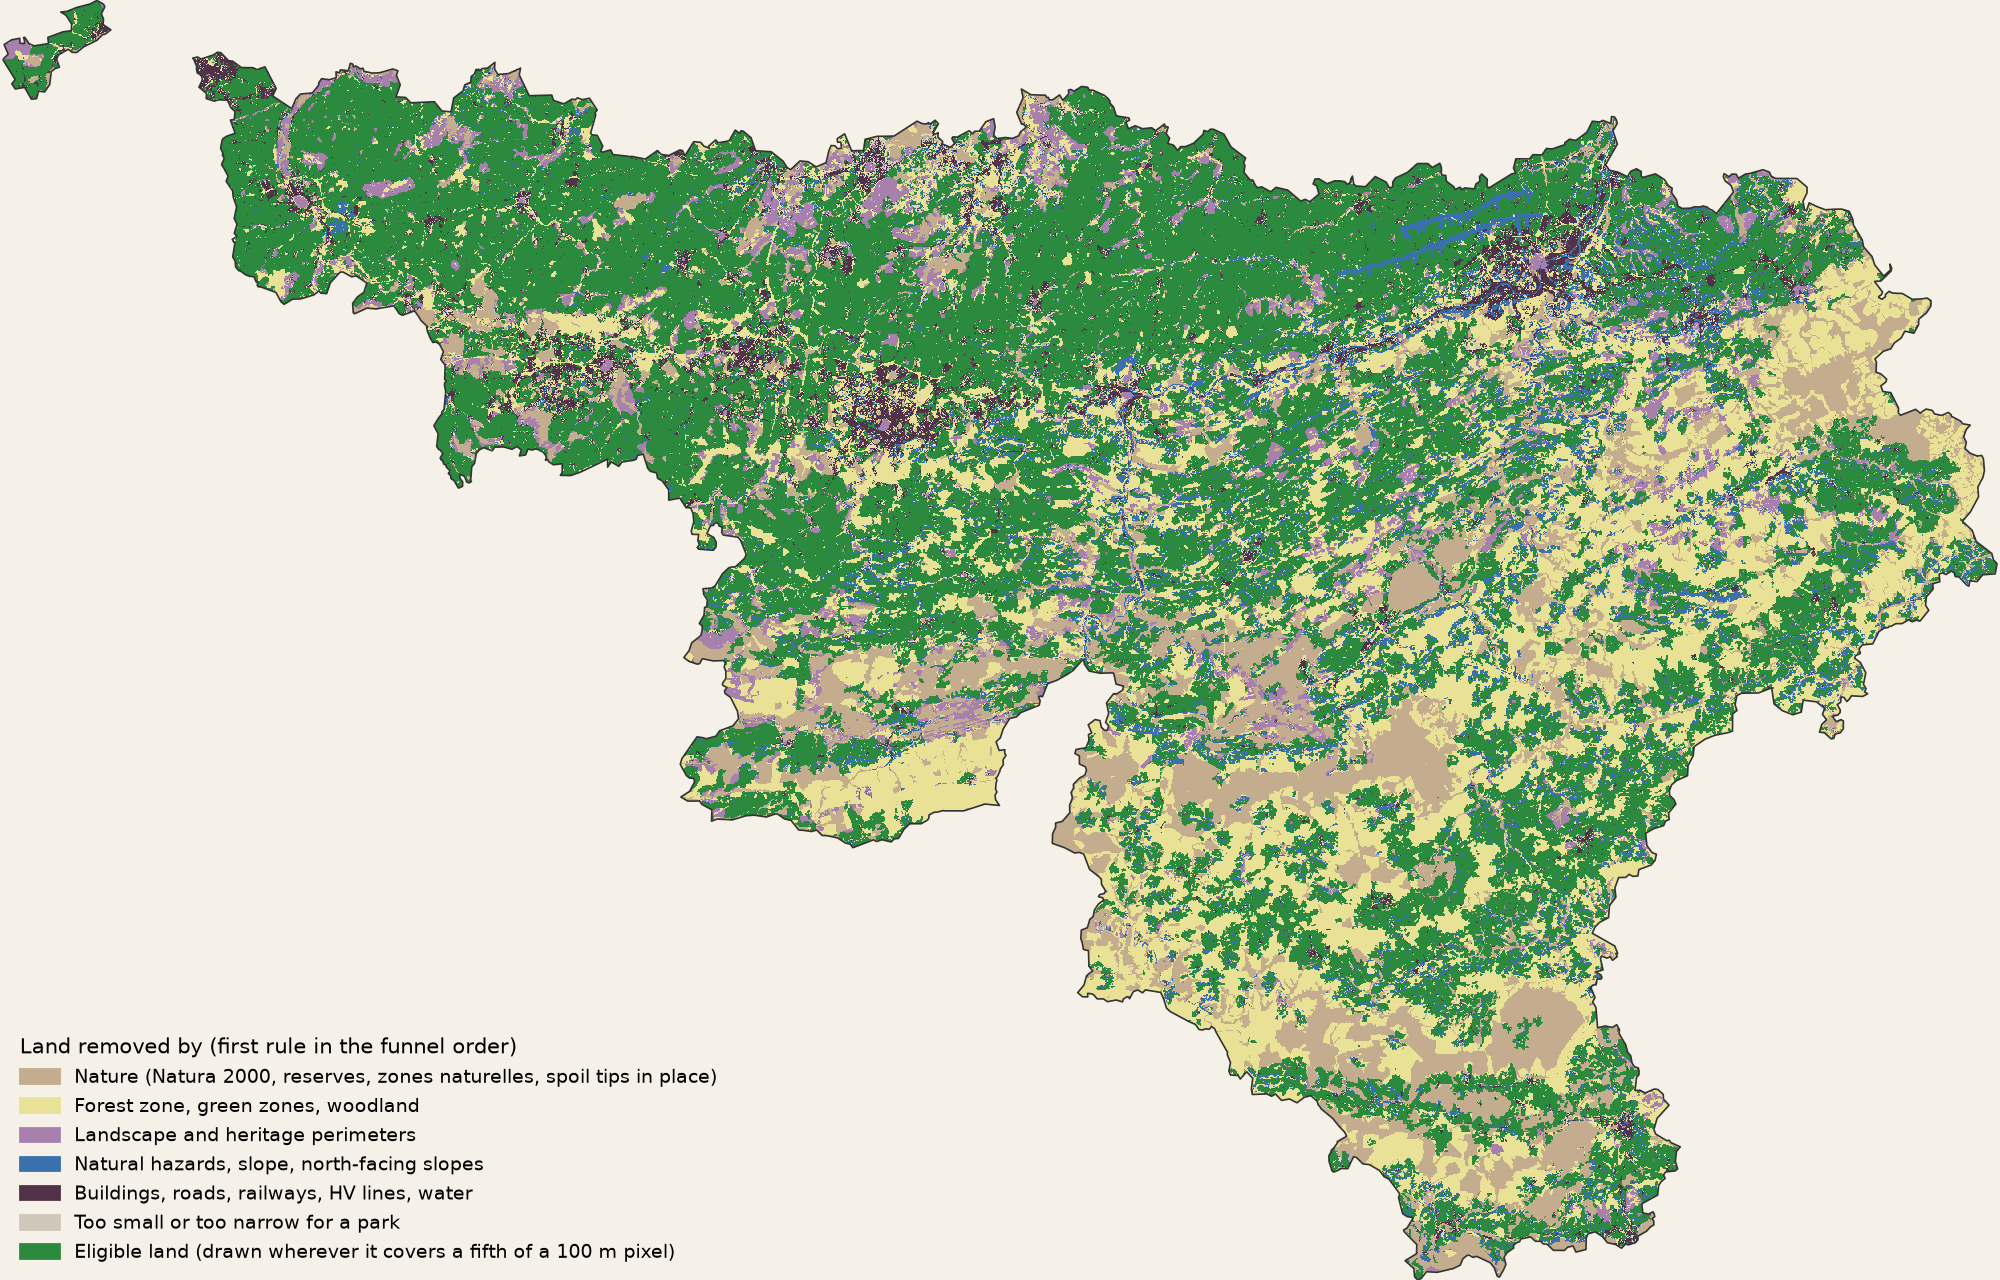
\includegraphics[width=\linewidth]{figures/map_exclusions.png}
\caption{The first family of rules that removes each piece of land, and the
land that survives the park rule.}\label{fig:exclusions}
\end{figure}

\begin{table}[htbp]
\centering\small
\caption{Land left after each family, in the order applied.}\label{tab:funnel}
\begin{tabular}{lrr}
\toprule
step & km\textsuperscript{2} left & \% of the Region \\
\midrule
Walloon Region & \RegionKm & 100 \\
$-$ nature & \LeftNatureKm & \LeftNaturePct \\
$-$ forest and green zones & \LeftForestKm & \LeftForestPct \\
$-$ woodland (land cover) & \LeftCoverKm & \LeftCoverPct \\
$-$ landscape and heritage & \LeftLandscapeKm & \LeftLandscapePct \\
$-$ natural hazards & \LeftHazardKm & \LeftHazardPct \\
$-$ slope and north-facing slopes & \LeftTerrainKm & \LeftTerrainPct \\
$-$ buildings and networks & \LeftBuiltKm & \LeftBuiltPct \\
$-$ water & \LeftWaterKm & \LeftWaterPct \\
$-$ park rule (\ParkMinHa~ha, \ParkMinWidth~m) & \LeftParkRuleKm & \LeftParkRulePct \\
\bottomrule
\end{tabular}
\end{table}

\begin{figure}[htbp]
\centering
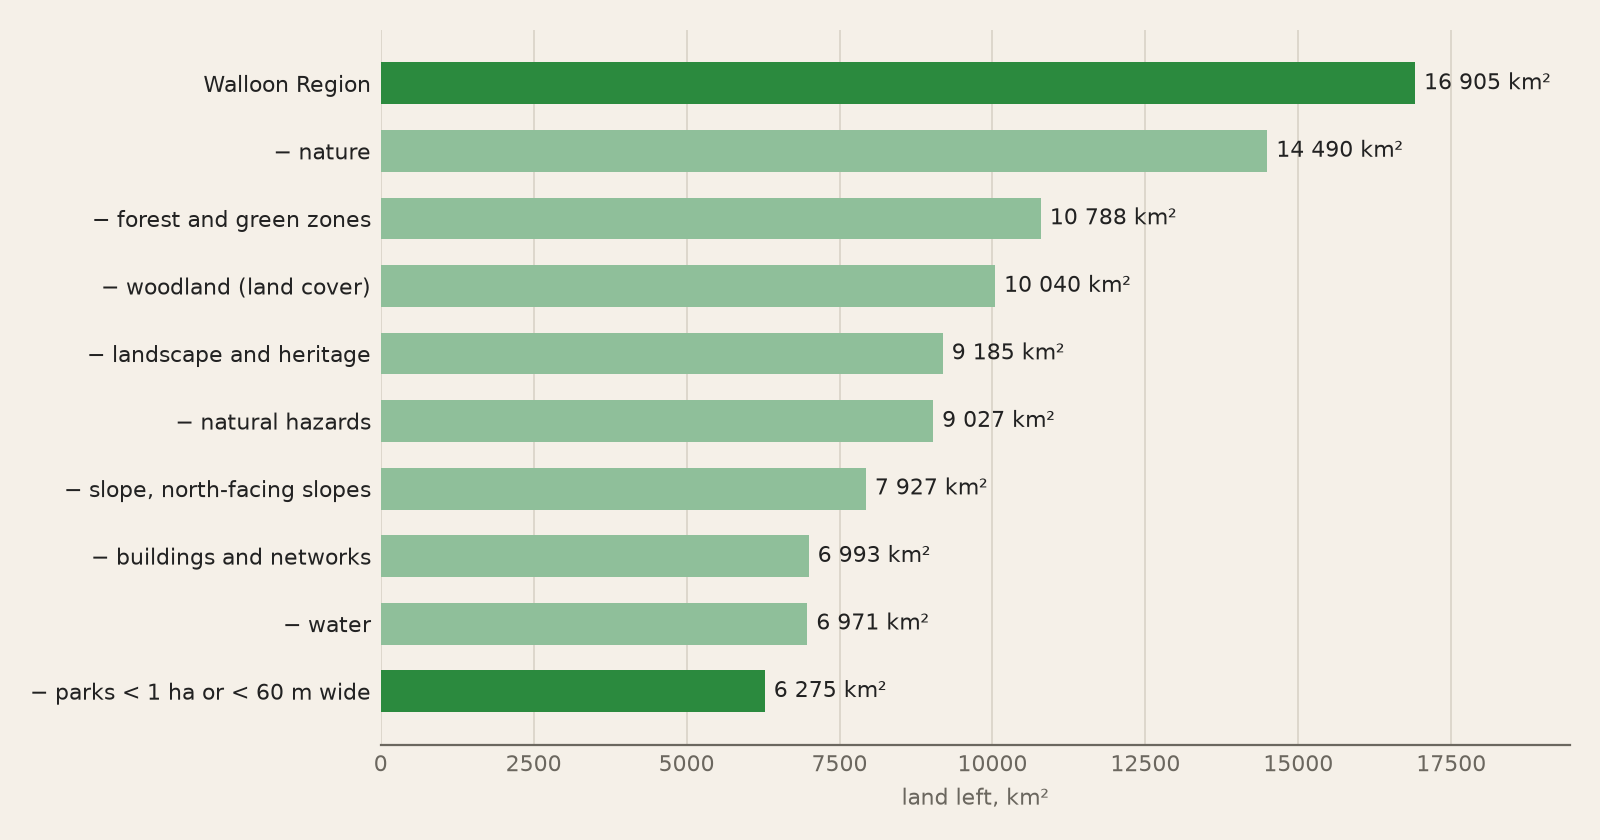
\includegraphics[width=0.85\linewidth]{figures/funnel.png}
\caption{Land left after each family of rules.}\label{fig:funnel}
\end{figure}

\subsection{What the land is}

Almost all of the land left is farmland (Table~\ref{tab:gisements},
Figures~\ref{fig:gisements} and~\ref{fig:gisbars}): \GAgriGrasslandPermTechHa{}~ha
of permanent grassland, \GAgriArableTechHa{}~ha of arable land. The degraded
categories are small by comparison: \GSarTechHa{}~ha of brownfields after
exclusions and the park rule --- the SAR perimeters carry buildings, woodland and
slopes --- \GExtractionTechHa{}~ha of unexploited extraction zones, \GCetTechHa{}~ha
of landfills, \GInfraEdgeTechHa{}~ha of verges before the park rule is re-applied
to them alone (\GInfraEdgeOpenHa{}~ha after), and \GWaterIndustrialTechHa{}~ha of
industrial basins and quarry lakes. The free land of the activity and
public-service zones (\GZaeTechHa{} and \GZspecTechHa{}~ha) is the largest
non-agricultural reserve, and a quarter of it is opened.

\begin{figure}[htbp]
\centering
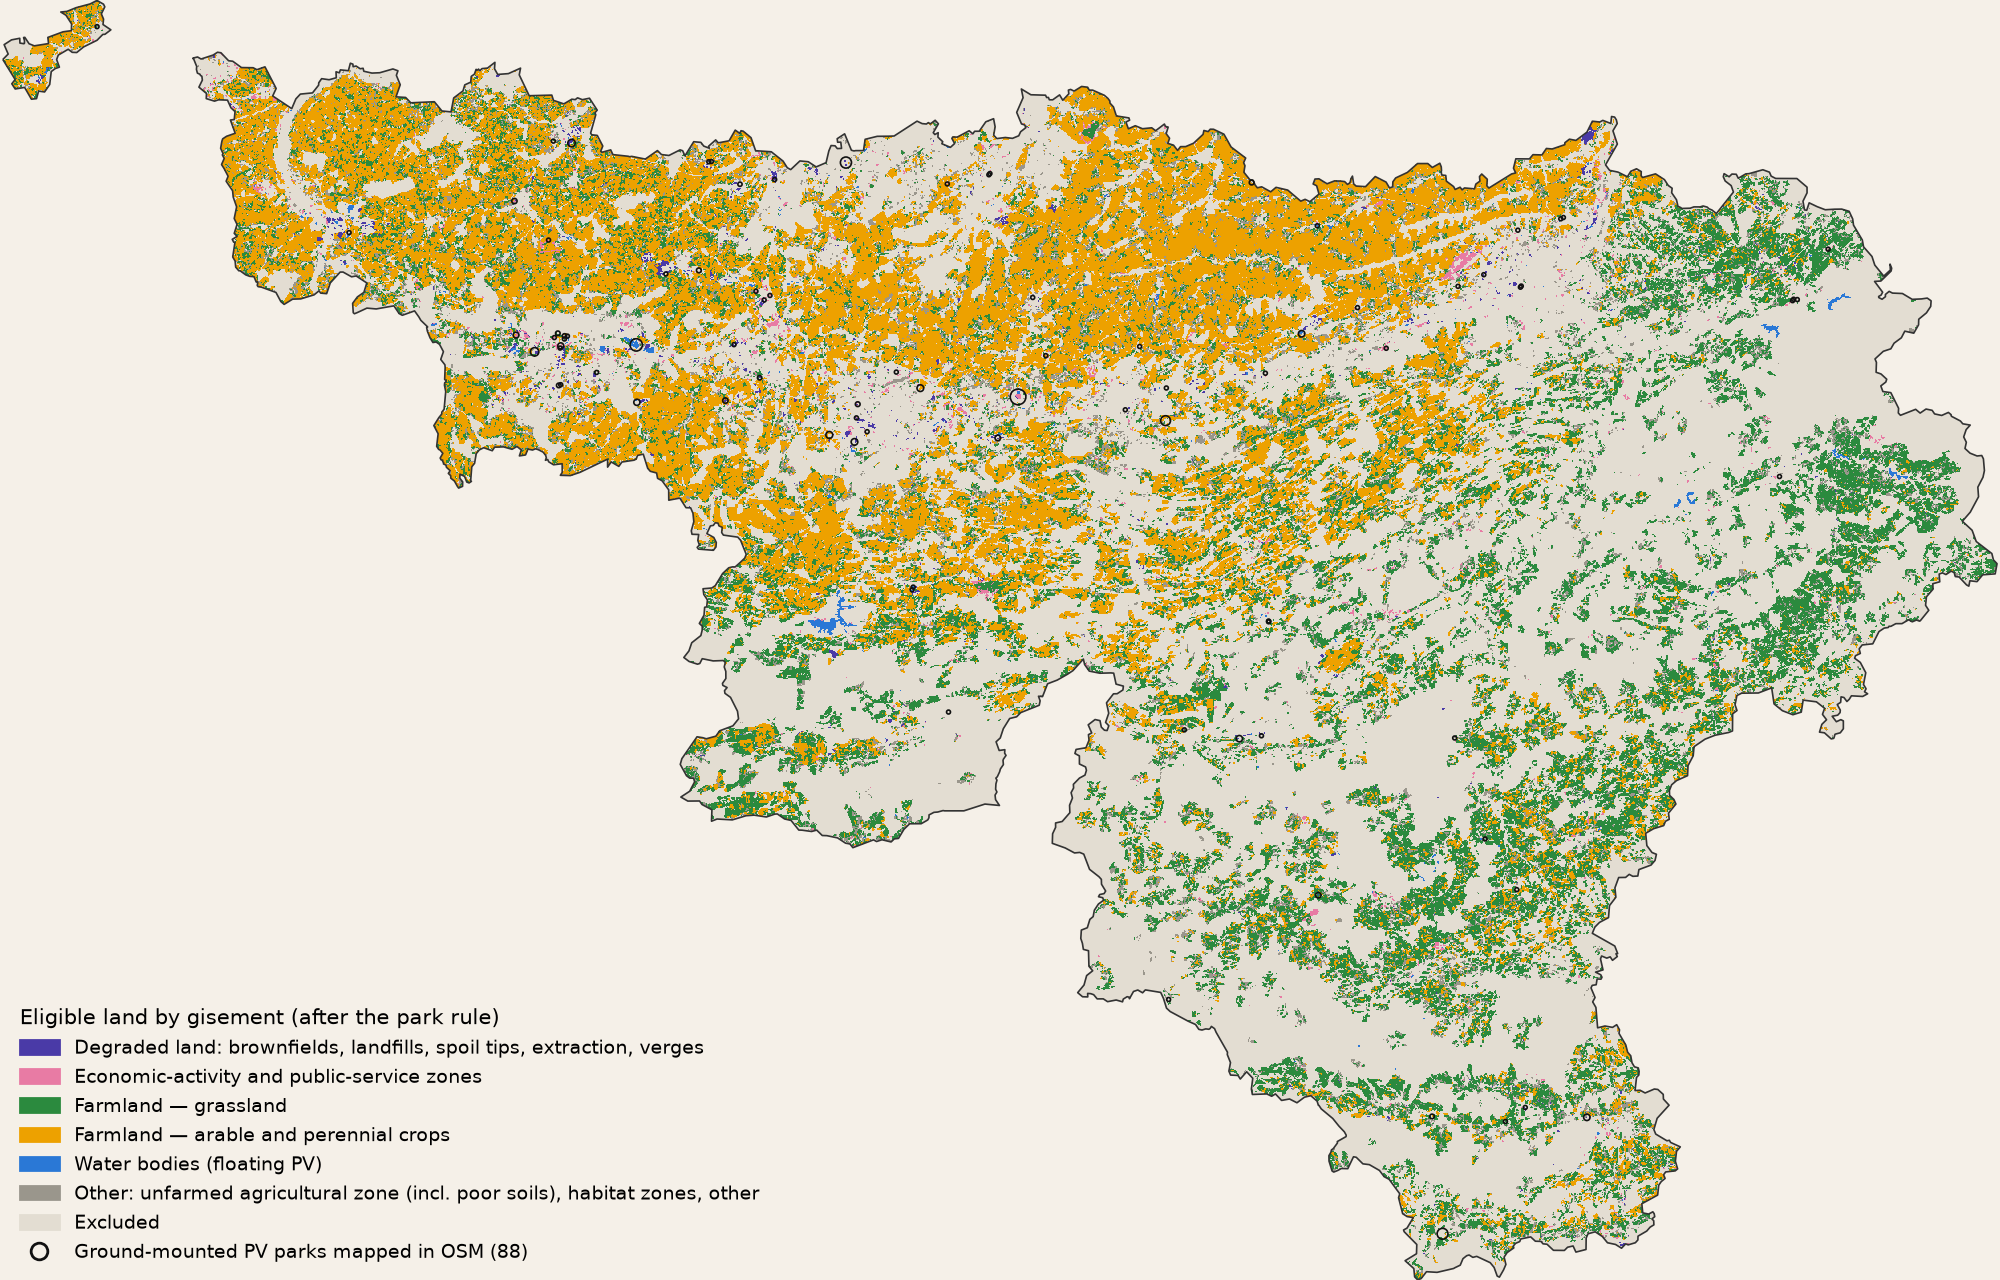
\includegraphics[width=\linewidth]{figures/map_gisements.png}
\caption{Eligible land after the park rule, by gisement group, and the
ground-mounted parks of OSM.}\label{fig:gisements}
\end{figure}

\begin{table}[htbp]
\centering\small
\caption{Gisements: eligible land, land after the park rule, technical
capacity, and what the reference opens. Open share in \%; the reference
capacity is computed on the park rule re-applied to the opened land.}\label{tab:gisements}
\resizebox{\linewidth}{!}{%
\begin{tabular}{llrrrrrr}
\toprule
gisement & system & eligible ha & after park rule ha & MWc/ha & technical MWc & open \% & reference MWc \\
\midrule
\tablefile{generated/table_gisements.tex}
\bottomrule
\end{tabular}}
\end{table}

\begin{figure}[htbp]
\centering
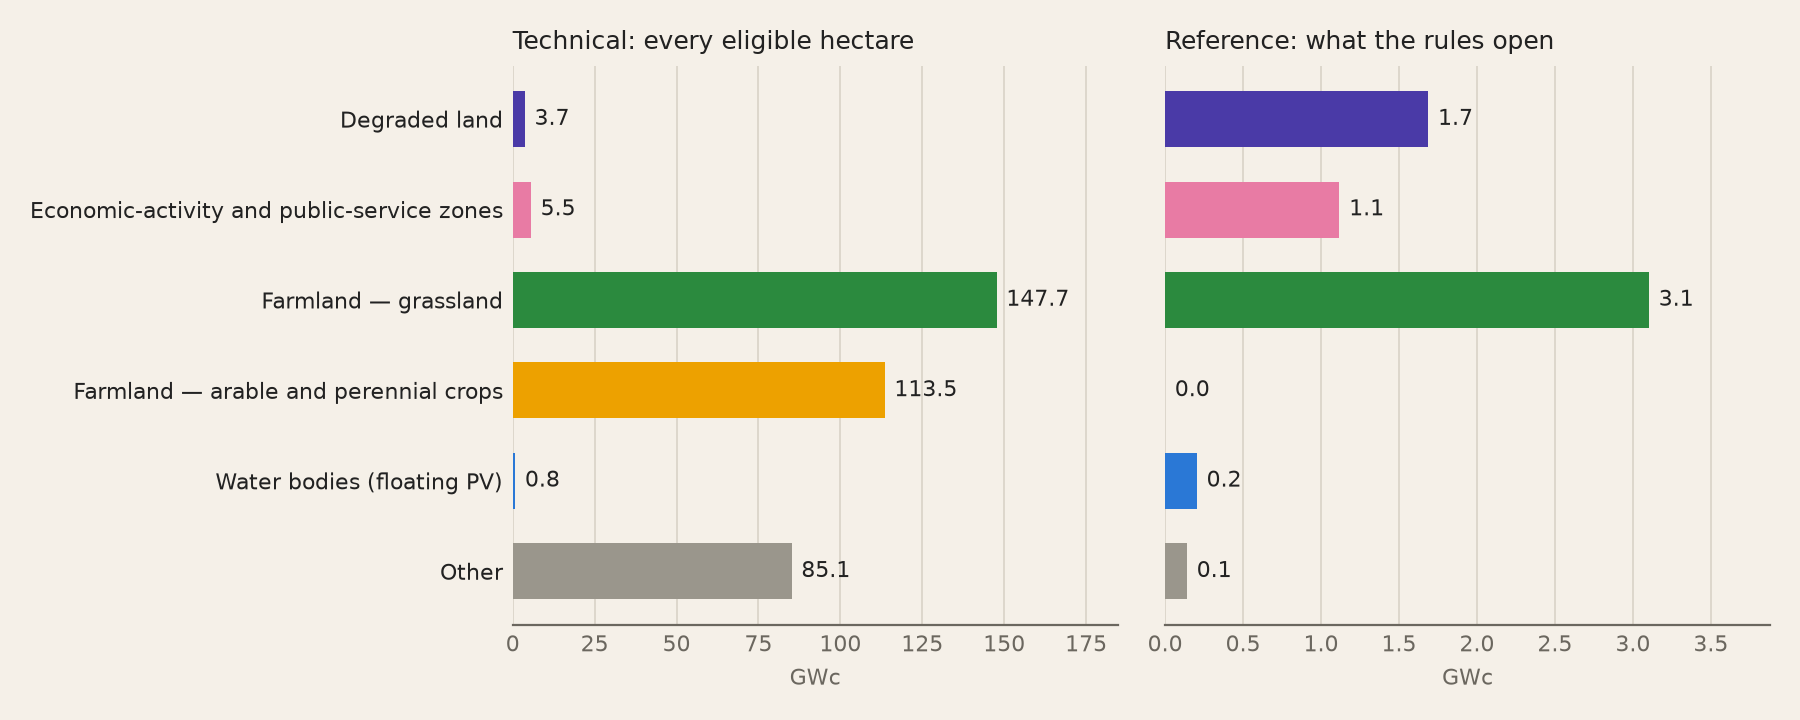
\includegraphics[width=\linewidth]{figures/gisements.png}
\caption{Capacity by gisement group: technical, and what the reference opens.}\label{fig:gisbars}
\end{figure}

\finding{The land is not the constraint: \TechGW{}~GWc of technical potential,
of which \TechAgriGW{}~GWc on declared farmland and \TechNonAgriGW{}~GWc on
everything else. The reference opens \RefGW{}~GWc, about \RefTWh{}~TWh a year:
\RefNonAgriGW{}~GWc off the farmland and \RefAgriGW{}~GWc of agrivoltaics.}

% =====================================================================
\section{What the answer depends on}\label{sec:sensitivity}

Every case is the reference with one change (Table~\ref{tab:sensitivity},
Figure~\ref{fig:sensitivity}).

\begin{longtable}{p{9.3cm}rrr}
\caption{Every choice priced one at a time against the reference
(\RefMW{}~MWc).}\label{tab:sensitivity}\\
\toprule
case & MWc & $\Delta$ MWc & $\Delta$ \% \\
\midrule
\endfirsthead
\toprule
case & MWc & $\Delta$ MWc & $\Delta$ \% \\
\midrule
\endhead
\tablefile{generated/table_sensitivity.tex}
\bottomrule
\end{longtable}

\begin{figure}[htbp]
\centering
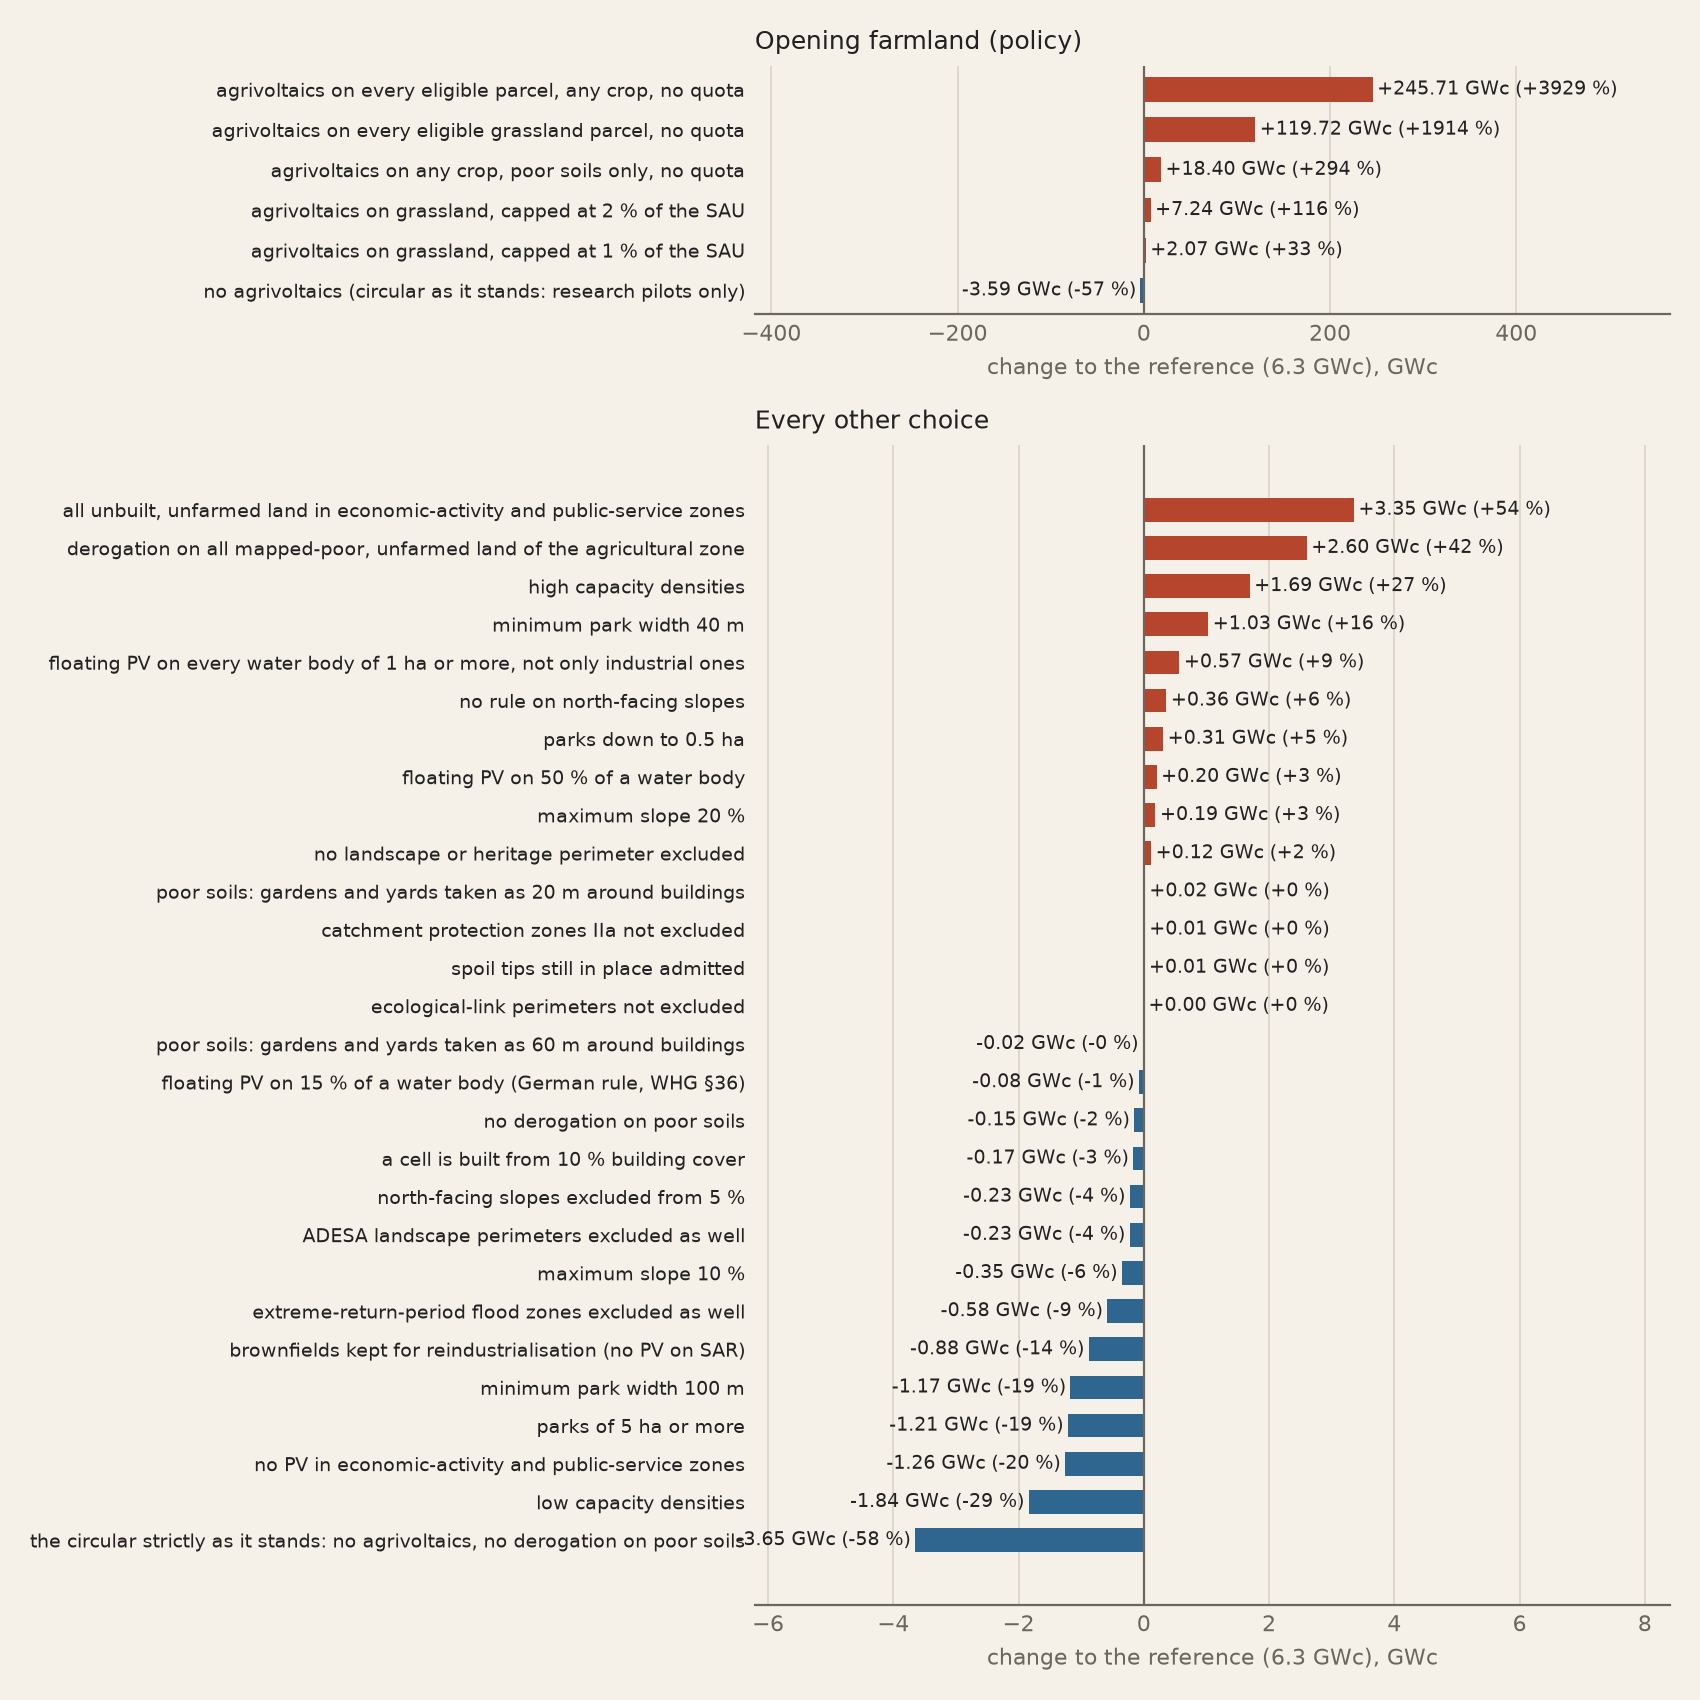
\includegraphics[width=0.95\linewidth]{figures/sensitivity.png}
\caption{Every choice as a change to the reference. Farmland on its own axis:
it is an order of magnitude larger than every other choice.}\label{fig:sensitivity}
\end{figure}

\subsection{Farmland decides}

The reference carries agrivoltaics on \RefAgriHa{}~ha, 0.6\,\% of the
agricultural area, \RefAgriGW{}~GWc. Closing them (the circular as it stands:
research pilots only) changes the reference by \SAgriClosedDeltaGW{}~GWc; a quota
at 1\,\% gives \SAgriQuotaOneGW{}~GWc, at 2\,\% \SAgriQuotaTwoGW{}. Beyond, only a
policy choice, not land, sets the answer: every eligible grassland parcel gives
\SAgriGrasslandAllGW{}~GWc, every eligible parcel \SAgriAllGW{}~GWc. Restricting
agrivoltaics to the parcels mapped on poor soils, without quota, gives
\SAgriPoorSoilsGW{}~GWc. The Livre blanc's 0.6\,\% is the land the PV still to
be built to 2030 would take if all of it were agrivoltaic; for 2050 it is a low
reading.

\subsection{The other policy choices}

Keeping the brownfields for reindustrialisation costs \SSarReservedPct{}\,\%;
closing the activity zones \SZaeClosedPct{}\,\%, opening all their free land
\SZaeOpenPct{}\,\%; floating PV on every water body \SWaterOpenPct{}\,\%. On the
poor soils, no derogation at all changes the reference by
\SPoorSoilsNoneDeltaGW{}~GWc and the derogation on all of them by
\SPoorSoilsAllDeltaGW{}~GWc; the curtilage distance at 20 or 60~m by
\SCurtilageTwoZeroPct{} and \SCurtilageSixZeroPct{}\,\%.

\subsection{Judgements and technical criteria}

None changes the order of magnitude, but two matter: the park rule (a 5~ha
minimum \SParkFivehaPct{}\,\%, a 100~m width \SWidthOneZeroZeroPct{}\,\%, 40~m
\SWidthFourZeroPct{}\,\%) and the densities. The others are smaller: the landscape
perimeters (\SNoLandscapePct{}\,\% if none is excluded), the slope threshold
(\SSlopeOneZeroPct{}\,\% at 10\,\%, \SSlopeTwoZeroPct{}\,\% at 20\,\%), the park size
(\SParkZeroFivehaPct{}\,\% down to 0.5~ha, \SParkFivehaPct{}\,\% from 5~ha), and the
densities (\SDensityLowPct{} / \SDensityHighPct{}\,\%).

% =====================================================================
\section{Against the other estimates}\label{sec:comparison}

\begin{itemize}
\item \textbf{APERe (2020)}: brownfields ``$\geq$~\ApereGW{}~GWc''. This study
  opens \GSarRefMW{}~MWc on the SAR inventories after exclusions and the park rule
  --- brownfields carry buildings, woodland and slopes, and a large part of their
  area is not free.
\item \textbf{Livre blanc (2024)}: 0.6\,\% of the agricultural area for the
  PV still to be built to 2030 --- the reference's agrivoltaic quota; the GLAES areas (\GlaesOneHa{} to
  \GlaesThreeHa{}~ha) are of the same order as this study's eligible grassland,
  and the quota, not the land, is what binds.
\item \textbf{PACE 2030}: \PaceGWh{}~GWh of PV, about \PaceGW{}~GWc, all
  segments together, against \InstalledGW{}~GWc installed at the end of 2025,
  mostly on roofs. The ground-mounted reference, \RefGW{}~GWc, is of the same
  order as the whole 2030 increment.
\item \textbf{PyPSA-Eur}: \PypsaEurGW{}~GW, a land bound that admits farmland and
  ignores the plan de secteur.
\end{itemize}

% =====================================================================
\section{What this means for \texttt{p\_nom\_max}}\label{sec:model}

The model's \ModelCapGW{}~GW is not contradicted by land: \TechGW{}~GWc of
technical potential remain. It is a policy assumption --- in effect, the
reference with agrivoltaics on 2\,\% of the agricultural area rather than
0.6\,\% --- and should be documented as such rather than as the sum of two
estimates. The workflow gives the number any such assumption implies:

\begin{center}\small
\begin{tabular}{lr}
\toprule
assumption & GWc \\
\midrule
circular strictly as it stands (no derogation, no agrivoltaics) & \SRulesInForceGW \\
\textbf{reference}: $+$ demonstrable poor soils, agrivoltaics 0.6\,\% of the SAU & \textbf{\RefGW} \\
reference with agrivoltaics at 1\,\% of the SAU & \SAgriQuotaOneGW \\
reference with agrivoltaics at 2\,\% of the SAU & \SAgriQuotaTwoGW \\
model cap today & \ModelCapGW \\
\bottomrule
\end{tabular}
\end{center}

A scenario dimension on the farmland rule, rather than one cap, would make the
choice visible in the model's results. No PyPSA-Wal input has been modified.

% =====================================================================
\section{Hypotheses and limits}\label{sec:gaps}

\begin{itemize}
\item \textbf{Not represented}: the SGIB (not published as a layer), the
  \emph{périmètres de point de vue remarquable} (published empty), the grid
  capacity, the BDES (restricted licence).
\item \textbf{The activity-zone share} (a quarter) is a judgement: the circular
  gives no figure, and the free land of an activity zone is also its reserve
  for firms.
\item \textbf{Brownfields} are counted as open although the circular admits PV
  there only temporarily; a temporary park still counts for a 2050 capacity.
\item \textbf{WALOUS 2023} decides what is built and what is woodland at 1~m;
  its classification errors (young plantations, glasshouses) pass into the
  result at the 20~m cell.
\item \textbf{The OSM inventory} is incomplete and is used for calibration only.
\end{itemize}

% =====================================================================
\section{Data provenance}\label{sec:sources}

\begin{longtable}{p{6.2cm}p{5.2cm}rr}
\toprule
dataset & service / layer & features & retrieved \\
\midrule
\endhead
\tablefile{generated/table_sources.tex}
SIGEC 2024 parcels (bulk GeoPackage) & SPW, CC-BY & & 2026-09-29 \\
WALOUS 2023 land cover, 1~m & SPW, CC-BY & & 2026-09-29 \\
LiDAR terrain model 2021--22, 1~m & SPW, CC-BY & & 2026-09-29 \\
Soil agronomic quality (AWAC/GxABT) & SPW, CC-BY & & 2026-09-29 \\
Ground-mounted PV parks, substations & OpenStreetMap, ODbL & \FleetN & 2026-09-29 \\
\bottomrule
\end{longtable}

\end{document}
